%\documentclass[mathserif]{beamer}              %use this for creating the presentation
\documentclass[handout,mathserif]{beamer}       %use this for creating the handout (i.e. no animation)
\usepackage{amsmath}
\usepackage{amssymb}
\usepackage{amsthm}
\usepackage{graphicx}
%\usepackage{subfig}

\usecolortheme{orchid}

\newcommand{\alignbox}[1]
    {\begin{equation*} \boxed{ \begin{aligned} #1
    \end{aligned} } \end{equation*}}
\newcommand{\gatherbox}[1]
    {\begin{equation*} \boxed{ \begin{gathered} #1
    \end{gathered} } \end{equation*}}
\newcommand{\ejw}{e^{j\omega}}
\newcommand{\drm}{\textrm{d}}
\newcommand{\paused}{\vspace*{-\baselineskip}\pause}     %use this if \pause puts too much space before the next line

%\input{../commands}
%\setkeys{Gin}{draft=true}

\linespread{1.3}

\title{ME 233 -- Advanced Control II\\
    Lecture 25 \\
    Stability Analysis of a \\
    Direct Adaptive Control System}
\author{Tony Kelman}
\institute{UC Berkeley}


\begin{document}

\maketitle

\begin{frame}
    \frametitle{Outline}
    \tableofcontents
\end{frame}

\section{Review of direct adaptive control}
\begin{frame}
    \frametitle{Outline}
    \tableofcontents[currentsection]
\end{frame}

\begin{frame}
    \frametitle{Deterministic SISO ARMA model}

    SISO ARMA plant model:
    \begin{equation*}
        A(q^{-1}) y(k) = q^{-\drm} B(q^{-1}) u(k)
    \end{equation*}
    where $y(k)$ and $u(k)$ are scalar

    \begin{itemize}
        \item
        $u(k)$ is the control input

        \item
        $y(k)$ is the output

        \item
        $\drm$ is the pure time delay

        \item
        no disturbance
    \end{itemize}
\end{frame}

\begin{frame}
    \frametitle{Model assumptions}

    SISO ARMA plant model:
    \begin{equation*}
        A(q^{-1}) y(k) = q^{-\drm} B(q^{-1}) u(k)
    \end{equation*}
    where $y(k)$ and $u(k)$ are scalar

    \begin{itemize}
        \item
        The polynomials
        \begin{align*}
            A(q^{-1}) & = {\color{red} 1} + a_1 q^{-1} + \cdots + a_n q^{-n} \\
            B(q^{-1}) & = b_0 + b_1 q^{-1} + \cdots + b_m q^{-m}
        \end{align*}
        are co-prime

        \item
        $B(q^{-1})$ is anti-Schur

        \item
        $m$, $n$, and $\drm$ are known

        \item
        $0 < b_{mino} \leq b_0$, where $b_{mino}$ is known
    \end{itemize}
\end{frame}

\begin{frame}
    \frametitle{Control Objectives}
    \begin{enumerate}
        \item[1.]
        \textbf{Pole Placement: } The poles of the closed-loop system must be placed at specific locations in the complex plane

        $ \ $
        \pause

        Closed-loop polynomial:
        \begin{align*}
            A_c(q^{-1}) = B(q^{-1}) A_c^{'}(q^{-1})
        \end{align*}
        where $A_c^{'}(q^{-1})$ is an anti-Schur polynomial chosen by the designer:
        \begin{align*}
            A_c^{'}(q^{-1}) & = {\color{red} 1} + a_{c1}^{'} q^{-1} + \cdots + a_{c(n_c')}^{'} q^{-(n_c')}
        \end{align*}
    \end{enumerate}

\end{frame}

\begin{frame}
    \frametitle{Control Objectives}
    \begin{enumerate}
        \item[2.]
        \textbf{Tracking: } The output sequence $y(k)$ must follow an arbitrary bounded reference sequence $y_d(k)$, which is known

        $ \ $
        \pause

        $y_d(k)$ is generated by the reference model
        \begin{align*}
            {\color{red} A_c^{'}(q^{-1})} y_d(k) = {\color{red}q^{-\drm}} B_m(q^{-1}) u_d(k)
        \end{align*}
        where
        \begin{itemize}
            \item
            $u_d(k)$ is a known \underline{bounded} reference input control input sequence

            \item
            $B_m(q^{-1})$ is chosen by the designer
        \end{itemize}

        $ \ $
        \pause

        Note that $A_c^{'}(q^{-1})$ comes from the pole placement and the reference model delay is the same as the plant delay
    \end{enumerate}
\end{frame}

\begin{frame}
    \frametitle{Reformulated plant dynamics}

    Using the solution of the Diophantine equation
    \begin{equation*}
        A_c^{'}(q^{-1}) = A(q^{-1}) R^{'}(q^{-1}) + q^{-\drm} S(q^{-1})
    \end{equation*}
    we rewrite the plant dynamics as
    \begin{align*}
        A_c^{'}(q^{-1}) y(k) = q^{-\drm} \Big[ R(q^{-1}) u(k) + S(q^{-1}) y(k) \Big]
    \end{align*}
    \pause

    where $R(q^{-1}) = R^{'}(q^{-1}) B(q^{-1})$ and
    \begin{align*}
        R(q^{-1}) & = r_0 + r_1 q^{-1} + \cdots + r_{n_r} q^{-n_r} \\
        S(q^{-1}) & = s_0 + s_1 q^{-1} + \cdots + s_{n_s} q^{-n_s}
    \end{align*}
    \begin{align*}
        n_r & = m + \drm - 1
            & n_s & = \max \{ n-1, n_c' - \drm \}
    \end{align*}

\end{frame}

\begin{frame}
    \frametitle{Reformulated plant dynamics}

    So far, we know that
    \begin{align*}
        A_c^{'}(q^{-1}) y(k) & = q^{-\drm} \Big[ R(q^{-1}) u(k) + S(q^{-1}) y(k) \Big] \\
        R(q^{-1}) & = r_0 + r_1 q^{-1} + \cdots + r_{n_r} q^{-n_r} \\
        S(q^{-1}) & = s_0 + s_1 q^{-1} + \cdots + s_{n_s} q^{-n_s}
    \end{align*}

    Defining $\eta(k) = A_c^{'}(q^{-1}) y(k)$ and
    \begin{align*}
        \phi(k) & = \begin{bmatrix}
                y(k) & \cdots & y(k-n_s) & u(k) & \cdots & u(k-n_r)
            \end{bmatrix}^T \\
        \theta_c & = \begin{bmatrix}
                s_0 & \cdots & s_{n_s} & r_0 & \cdots & r_{n_r}
            \end{bmatrix}^T
    \end{align*}
    we rewrite the plant dynamics as
    \alignbox{
        \eta(k) = \phi^T(k-\drm) \theta_c
    }

\end{frame}

\begin{frame}
    \frametitle{Direct adaptive control approach}

    The plant dynamics are written as
    \begin{align*}
        \eta(k) = \phi^T(k-\drm) \theta_c
    \end{align*}

    \begin{itemize}
        \item
        $\eta(k)$ is the known ``filtered output''

        \item
        $\phi(k)$ is the known regressor vector

        \item
        $\theta_c$ is the \underline{unknown} parameter vector
        \pause

        $\Rightarrow$ we use RLS to estimate $\theta_c$
    \end{itemize}

\end{frame}

\begin{frame}
    \frametitle{Tracking control objective}

    We would like to achieve
    \begin{align*}
        \lim_{k \rightarrow \infty} \{ y(k) - y_d(k) \} = 0
    \end{align*}
    \pause

    Since $A_c^{'}(q^{-1})$ is anti-Schur this is equivalent to
    \begin{align*}
        0 & = \lim_{k \rightarrow \infty} \{ A_c^{'}(q^{-1}) [y(k) - y_d(k)] \} \\
        & = \lim_{k \rightarrow \infty} \{ \eta(k) - \eta_d(k) \}
    \end{align*}
    where $\eta_d(k) = A_c^{'}(q^{-1}) y_d(k) = q^{-\drm} B_m(q^{-1}) u_d(k) = r(k-\drm)$.
\end{frame}

\begin{frame}
    \frametitle{List of error signals}

    Parameter estimation error:
    \begin{align*}
        \tilde{\theta}_c(k) = \theta_c - \hat{\theta}_c(k)
    \end{align*}
    \pause
    Filtered output \underline{estimation} errors:
    \begin{align*}
        e^o(k) & = \eta(k) - \phi^T(k-\drm) \hat{\theta}_c(k-1)
            && \textrm{a-priori} \\
        & = \phi^T(k-\drm) \tilde{\theta}_c(k-1) \\
        e(k) & = \eta(k) - \phi^T(k-\drm) \hat{\theta}_c(k)
            && \textrm{a-posteriori} \\
        & = \phi^T(k-\drm) \tilde{\theta}_c(k)
    \end{align*}
    \pause
    Filtered output \underline{tracking} error:
    \begin{align*}
        \epsilon(k) & = \eta(k) - \eta_d(k)
    \end{align*}
\end{frame}

\begin{frame}
    \frametitle{Direct adaptive control}

    \begin{enumerate}
        \item
        $\eta(k+1) = A_c^{'}(q^{-1}) y(k+1)$

        \item
        $\phi(k-\drm+1) = \begin{bmatrix}
                y(k-\drm+1) \\
                \vdots \\
                y(k-\drm+1-n_s) \\
                u(k-\drm+1) \\
                \vdots \\
                u(k-\drm+1-n_r)
            \end{bmatrix}$

        \item
        $e^o(k+1) = \eta(k+1) - \phi^T(k-\drm+1) \hat{\theta}_c(k)$

        \item
        $\displaystyle e(k+1) = \frac{ \lambda_1(k) }
            { \lambda_1(k) + \phi^T(k-\drm+1) F(k) \phi(k-\drm+1) } e^o(k+1)$

        \item
        $\displaystyle \hat{\theta}_c^o(k+1) = \hat{\theta}_c(k) + \frac{1}{\lambda_1(k)} F(k) \phi(k-\drm+1) e(k+1)$
    \end{enumerate}
\end{frame}

\begin{frame}
    \frametitle{Direct adaptive control}

    \begin{enumerate}
        \item[6.]
        Form $\hat{\theta}_c(k+1)$: \\
        $\hat{s}_i(k+1) = \hat{s}_i^o(k+1), \quad i = 0,\ldots,n_s$ \\
        $\hat{r}_i(k+1) = \hat{r}_i^o(k+1), \quad i = 1,\ldots,n_r$ \\
        $\hat{r}_0(k+1) = \max \{ b_{mino}, \hat{r}_0^o(k+1) \}$ \hfill parameter projection

        $ \ $

        \item[7.]
        $\displaystyle F(k+1) = \frac{1}{\lambda_1(k)} \Bigg[ F(k)$ \\
        $\displaystyle \hspace{1.7cm} -\lambda_2(k) \frac{ F(k) \phi(k-\drm+1) \phi^T(k-\drm+1) F(k) } {\lambda_1(k) + \lambda_2(k) \phi^T(k-\drm+1) F(k) \phi(k-\drm+1) } \Bigg]$

        $ \ $

        where $\lambda_1(k)$ and $\lambda_2(k)$ are chosen so that
        \begin{align*}
            0 < \underline{\lambda}_1 \leq \lambda_1(k) & \leq 1
                & 0 \leq \lambda_2(k) \leq \overline{\lambda}_2 < 2
        \end{align*}
        and $0 < K_{min} \leq \lambda_{min}(F(k)) \leq \lambda_{max}(F(k)) \leq K_{max} < \infty$

    \end{enumerate}
\end{frame}

\begin{frame}
    \frametitle{Direct adaptive control}

    \begin{enumerate}
        \item[8.]
        Apply control
        \begin{figure}[h]
            \centering
            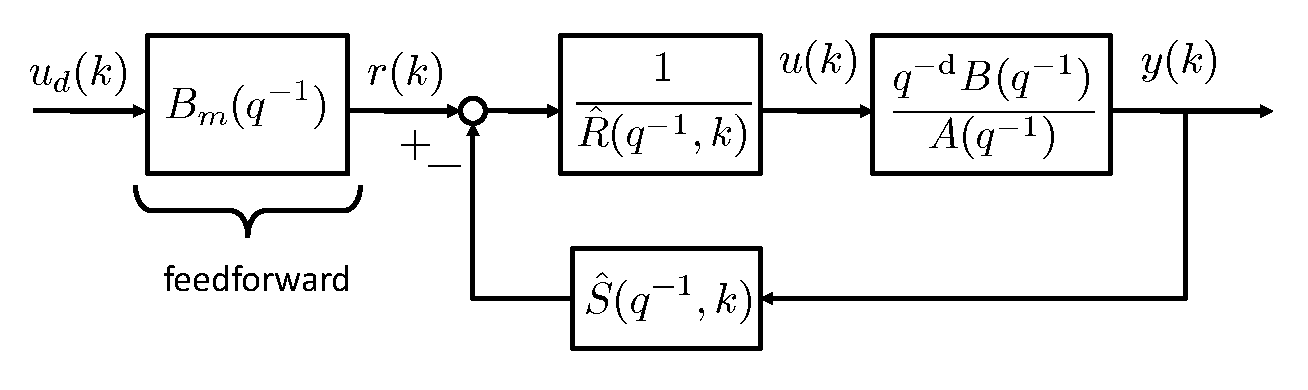
\includegraphics[width=8cm]{figs_control}\\
        \end{figure}
        \begin{align*}
            \hat{R}(q^{-1},k) u(k) = B_m(q^{-1}) u_d(k) - \hat{S}(q^{-1},k) y(k)
        \end{align*}
        where
        \begin{align*}
            \hat{R}(q^{-1},k) & = \hat{r}_0(k) + \hat{r}_1(k) q^{-1} + \cdots + \hat{r}_{n_r}(k) q^{-n_r} \\
            \hat{S}(q^{-1},k) & = \hat{s}_0(k) + \hat{s}_1(k) q^{-1} + \cdots + \hat{s}_{n_s}(k) q^{-n_s}
        \end{align*}

    \end{enumerate}
\end{frame}





\section{Stability theorem}
\begin{frame}
    \frametitle{Outline}
    \tableofcontents[currentsection]
\end{frame}

\begin{frame}
    \frametitle{Stability theorem}

    Using the direct adaptive control approach just outlined, the tracking error converges to zero, i.e.
    \alignbox{
        \lim_{k \rightarrow \infty} \epsilon(k) = 0
    }
    Moreover, $u(k)$ remains bounded, $e(k) \longrightarrow 0$, and $e^o(k)\longrightarrow 0$.
    \pause

    Note that the theorem \underline{does not} require:
    \begin{itemize}
        \item
        a-priori knowledge that the control input sequence $u(k)$ is bounded

        \item
        the polynomial $A(q^{-1})$ is anti-Schur

        \item
        any sort of persistence of excitation condition
    \end{itemize}
    \pause

    The theorem \underline{does not} state that the parameter estimates converge to the true values
\end{frame} 
\section{Stability theorem proof}
\begin{frame}
    \frametitle{Outline}
    \tableofcontents[currentsection]
\end{frame}

\begin{frame}
    \frametitle{Outline of stability theorem proof}

    \begin{enumerate}
        \item
        Use hyperstability theory to show that
        \begin{align*}
            \lim_{k \rightarrow \infty} e(k) = 0
        \end{align*}
        \pause

        \item
        Prove the limits
        \begin{gather*}
            \lim_{k \rightarrow \infty} \| \hat{\theta}_c(k) - \hat{\theta}_c(k-1) \| = 0 \\
            \lim_{k \rightarrow \infty} \frac{ [\lambda_1(k-1) e^o(k)]^2 }
                { \lambda_1(k-1) + \phi^T(k-\drm) F(k-1) \phi(k-\drm) } = 0 \\
            \lim_{k \rightarrow \infty} \frac{ [\lambda_1(k-1) \epsilon(k)]^2 }
                { \lambda_1(k-1) + \phi^T(k-\drm) F(k-1) \phi(k-\drm) } = 0
        \end{gather*}
    \end{enumerate}
\end{frame}

\begin{frame}
    \frametitle{Outline of stability theorem proof}

    \begin{enumerate}
        \item[3.]
        Prove that there exist $C_1 \geq 0, \ C_2 \geq 0$ such that
        \begin{align*}
            \| \phi(k-\drm) \| \leq C_1 + C_2 \max_{j \in \{0,\ldots,k\}} |\epsilon(j)|
        \end{align*}
        \pause

        \item[4.]
        Prove Goodwin's technical lemma, which states that $\| \phi(k) \|$ remains bounded and
        \begin{align*}
            \lim_{k \rightarrow \infty} \epsilon(k) = 0
        \end{align*}
        
        \item[5.]
        Prove that
        \begin{align*}
            \lim_{k \rightarrow \infty} e^o(k) = 0
        \end{align*}

    \end{enumerate}
\end{frame} 
\subsection{Part 1}
\begin{frame}
    \frametitle{Outline}
    \tableofcontents[currentsection]
\end{frame}

\begin{frame}
    \frametitle{Stability theorem proof, part 1}

    \begin{itemize}
        \item
        We want to show that $e(k) \rightarrow 0$

        \item
        Simplification: neglect parameter projection

        \item
        We will use hyperstability, as in Lecture 21
    \end{itemize}
\end{frame}

\begin{frame}
    \frametitle{Stability theorem proof, part 1}

    As in Lecture 21, the estimation error dynamics can be expressed using the block diagram
    \begin{figure}[h]
        \centering
        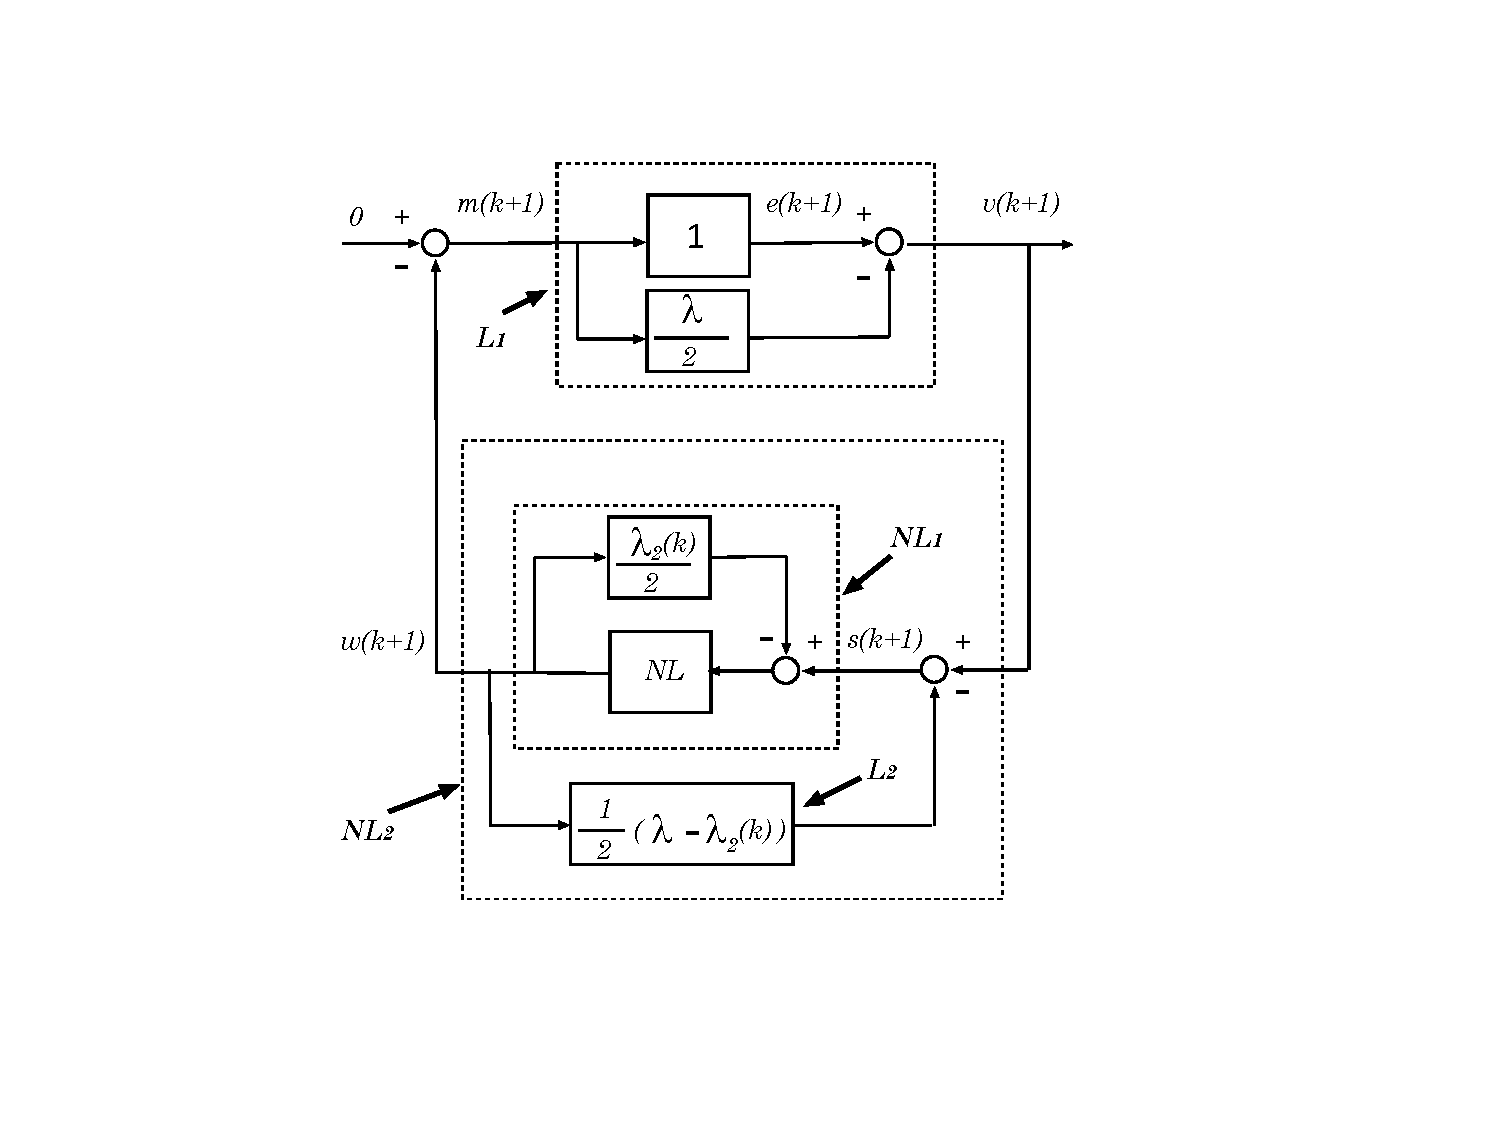
\includegraphics[width=6cm]{figs_hyperstability}\\
    \end{figure}
\end{frame}

\begin{frame}
    \frametitle{Stability theorem proof, part 1}

    We will now show that $NL_1$ is P-class:
    \begin{figure}[h]
        \centering
        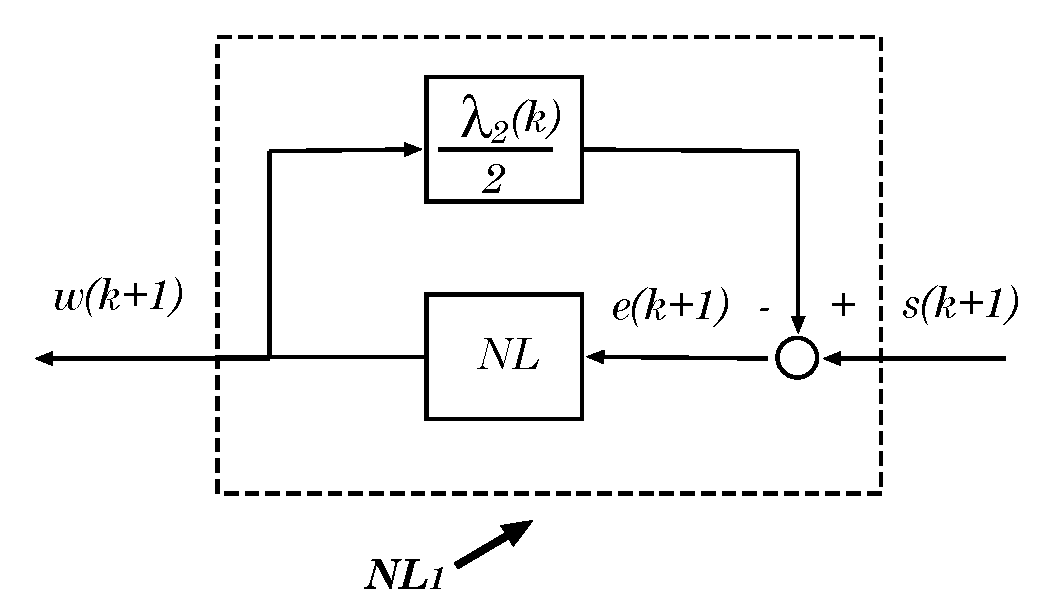
\includegraphics[width=5cm]{figs_NL1}\\
    \end{figure}
    \begin{align*}
        w(k) = -\phi^T(k-\drm) \tilde{\theta}_c(k)
    \end{align*}
    \pause

    Note that $\displaystyle e(k) = s(k) - \frac{\lambda_2(k-1)}{2} w(k)$, which implies that
    \begin{align*}
        s(k) = \frac{\lambda_2(k-1)}{2} w(k) + e(k)
    \end{align*}

\end{frame}

\begin{frame}
    \frametitle{Stability theorem proof, part 1}

    \begin{align*}
        2 w(k) s(k) & = w(k) \left[ {\color{red} \lambda_2(k-1) w(k)}
            + {\color{blue} 2 e(k)} \right] \\
        & = {\color{red} \lambda_2(k-1) \tilde{\theta}_c^T(k) \phi(k-\drm) \phi^T(k-\drm)
            \tilde{\theta}_c(k) } \\
        & \quad - {\color{blue} 2 \tilde{\theta}_c^T(k) [ \phi(k-\drm) e(k) ] } \\
        & = {\color{red} \tilde{\theta}_c^T(k) \Big[ \lambda_2(k-1) \phi(k-\drm) \phi^T(k-\drm) \Big]
            \tilde{\theta}_c(k) } \\
        & \quad - {\color{blue} 2 \tilde{\theta}_c^T(k) \left[ \lambda_1(k) F^{-1}(k-1)
            \Big( \tilde{\theta}_c(k-1) - \tilde{\theta}_c(k) \Big) \right] }
    \end{align*}
    \pause

    Define $\Delta \theta_c(k) = \hat{\theta}(k) - \hat{\theta}(k-1) = \tilde{\theta}_c(k-1) - \tilde{\theta}_c(k)$
    \pause
    \begin{align*}
        2 w(k) s(k) & = {\color{red} \tilde{\theta}_c^T(k)
            \Big[ F^{-1}(k) - \lambda_1(k) F^{-1}(k-1) \Big] \tilde{\theta}_c(k) } \\
        & \quad - {\color{blue} 2 \lambda_1(k) \tilde{\theta}_c^T(k) F^{-1}(k-1) \Delta \theta_c(k) }
    \end{align*}
\end{frame}

\begin{frame}
    \frametitle{Stability theorem proof, part 1}

    \vspace*{-\baselineskip}
    \begin{align*}
        2 w(k) s(k) & = {\color{red} \tilde{\theta}_c^T(k)
            \Big[ F^{-1}(k) - \lambda_1(k) F^{-1}(k-1) \Big] \tilde{\theta}_c(k) } \\
        & \quad - {\color{blue} 2 \lambda_1(k) \tilde{\theta}_c^T(k) F^{-1}(k-1) \Delta \theta_c(k) }
    \end{align*}
    \hrule{\hfill}
    
    \vspace*{-\baselineskip}
    \begin{align*}
        2 w(k) s(k) & = {\color{red} \tilde{\theta}_c^T(k) F^{-1}(k) \tilde{\theta}_c(k) }
            - \lambda_1(k) \Big[ {\color{red} \tilde{\theta}_c^T(k) F^{-1}(k-1) \tilde{\theta}_c(k) } \\
        & \quad {\color{blue} + 2 \tilde{\theta}_c^T(k) F^{-1}(k-1) \Delta\theta_c(k) } \Big] \\
        & = \tilde{\theta}_c^T(k) F^{-1}(k) \tilde{\theta}_c(k) \\
        & \quad - \lambda_1(k) \Big[ \Big( \tilde{\theta}_c(k) + \Delta\theta_c(k) \Big)^T
            F^{-1}(k-1) \Big( \tilde{\theta}_c(k) + \Delta\theta_c(k) \Big) \\
        & \quad - \Delta\theta_c^T(k) F^{-1}(k-1) \Delta\theta_c(k) \Big]
    \end{align*}
    \pause
    Note that $\tilde{\theta}_c(k) + \Delta \theta_c(k) = \tilde{\theta}_c(k-1)$
\end{frame}

\begin{frame}
    \frametitle{Stability theorem proof, part 1}

    From the previous slide,
    \begin{align*}
        2 w(k) s(k) & = \tilde{\theta}_c^T(k) F^{-1}(k) \tilde{\theta}_c(k)
            - \lambda_1(k) \tilde{\theta}_c^T(k-1) F^{-1}(k-1) \tilde{\theta}_c(k-1) \\
        & \quad + \lambda_1(k) \Delta\theta_c^T(k) F^{-1}(k-1) \Delta\theta_c(k)
    \end{align*}
    \pause
    
    Since $\lambda_1(k) \leq 1$ and $F(k-1) \succ 0$, this implies that
    \begin{align*}
         2 w(k) s(k) \geq \left[ \tilde{\theta}_c^T(k) F^{-1}(k) \tilde{\theta}_c(k)
            - \tilde{\theta}_c^T(k-1) F^{-1}(k-1) \tilde{\theta}_c(k-1) \right]
    \end{align*}
\end{frame}

\begin{frame}
    \frametitle{Stability theorem proof, part 1}

    \begin{align*}
         2 w(k) s(k) \geq \left[ \tilde{\theta}_c^T(k) F^{-1}(k) \tilde{\theta}_c(k)
            - \tilde{\theta}_c^T(k-1) F^{-1}(k-1) \tilde{\theta}_c(k-1) \right]
    \end{align*}
    \hrule{\hfill}
    
    Therefore
    \begin{align*}
        \Rightarrow \sum_{j=0}^k w(j) s(j) & \geq \frac{1}{2} \sum_{j=0}^k \Bigg[
            \tilde{\theta}_c^T(j) F^{-1}(j) \tilde{\theta}_c(j) \\
        & \quad - \tilde{\theta}_c^T(j-1) F^{-1}(j-1) \tilde{\theta}_c(j-1) \Bigg] \\
        & = \frac{1}{2} \Bigg[ \tilde{\theta}_c^T(k) F^{-1}(k) \tilde{\theta}_c(k)
            - \tilde{\theta}_c^T(-1) F^{-1}(-1) \tilde{\theta}_c(-1) \Bigg] \\
        & \geq - \frac{1}{2} \tilde{\theta}_c^T(-1) F^{-1}(-1) \tilde{\theta}_c(-1)
    \end{align*}
\end{frame}

\begin{frame}
    \frametitle{Stability theorem proof, part 1}

    \begin{columns}[c]
        \column{0.5\textwidth}
        We have shown that $NL_1$ is P-class

        $ \ $

        Using the same arguments as in Lecture 21 (including the asymptotic hyperstability theorem), this yields
        \alignbox{
            \lim_{k\rightarrow \infty} e(k) = 0
        }

        \column{0.5\textwidth}
        \begin{figure}[h]
            \centering
            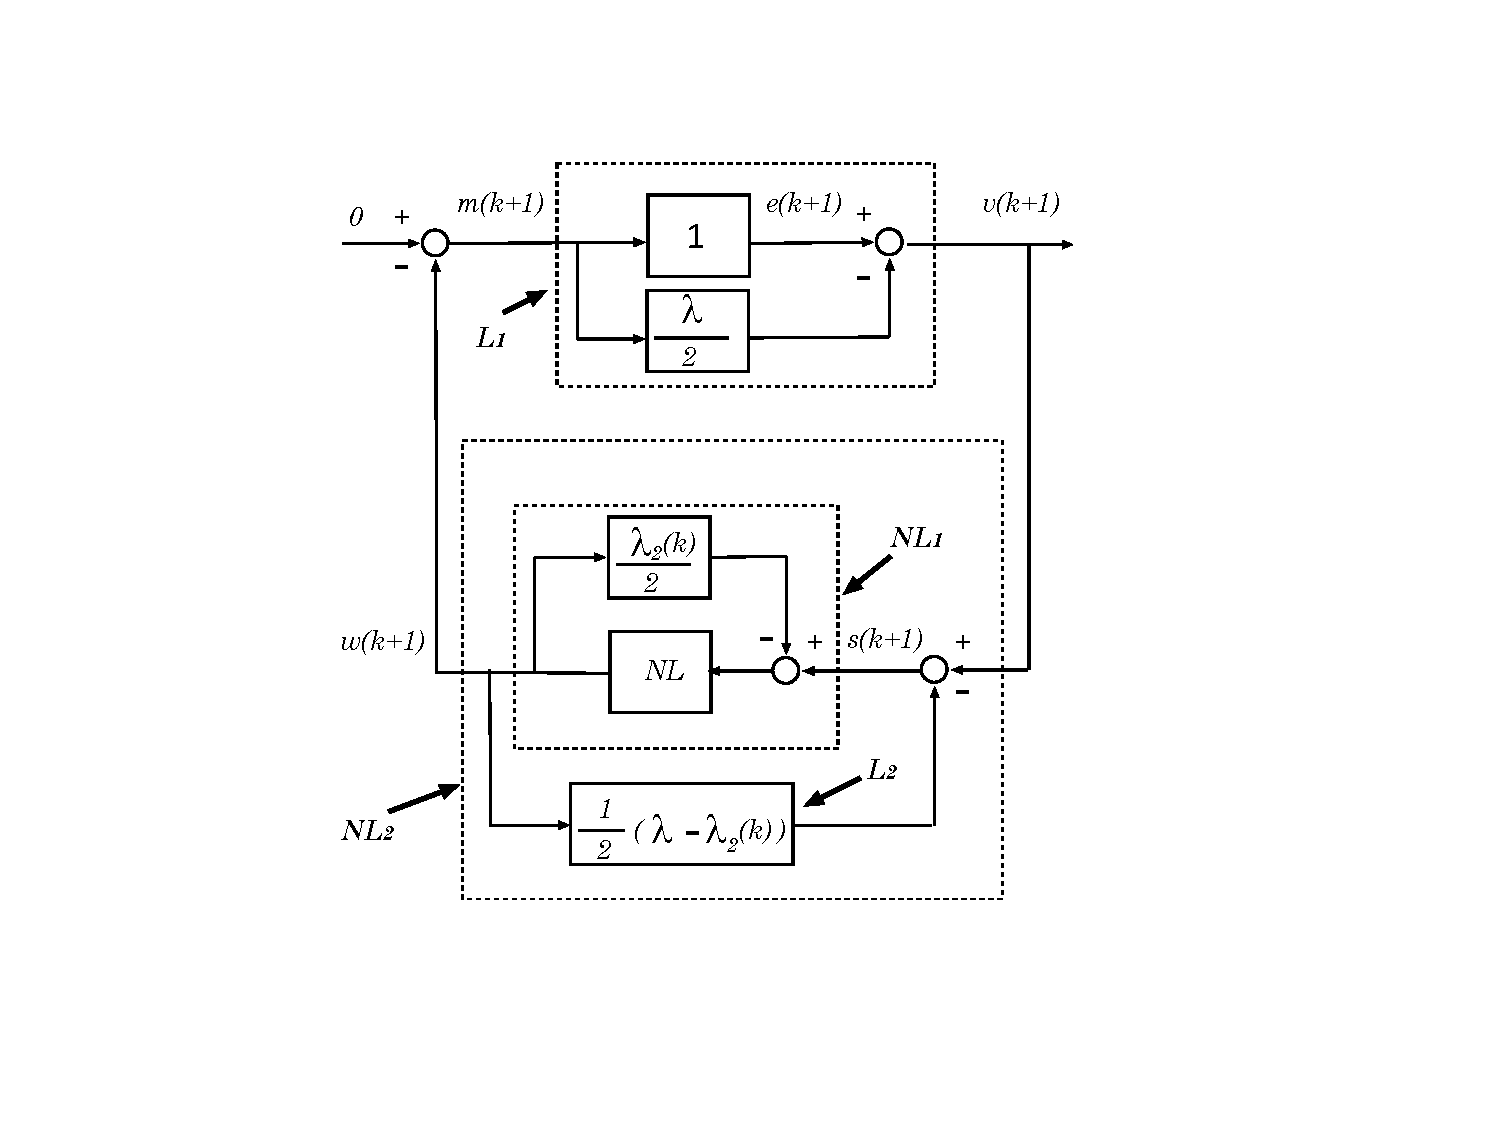
\includegraphics[width=5cm]{figs_hyperstability}\\
        \end{figure}
    \end{columns}

\end{frame}


\subsection{Part 2}
\begin{frame}
    \frametitle{Outline}
    \tableofcontents[currentsection]
\end{frame}

\begin{frame}
    \frametitle{Stability theorem proof, part 2}

    We want to prove the limits
    \begin{gather*}
        \lim_{k \rightarrow \infty} \| \hat{\theta}_c(k) - \hat{\theta}_c(k-1) \| = 0 \\
        \, \\
        \lim_{k \rightarrow \infty} \frac{ [\lambda_1(k-1) e^o(k)]^2 }
            { \lambda_1(k-1) + \phi^T(k-\drm) F(k-1) \phi(k-\drm) } = 0 \\
        \, \\
        \lim_{k \rightarrow \infty} \frac{ [\lambda_1(k-1) \epsilon(k)]^2 }
            { \lambda_1(k-1) + \phi^T(k-\drm) F(k-1) \phi(k-\drm) } = 0
    \end{gather*}
\end{frame}

\begin{frame}
    \frametitle{Stability theorem proof, part 2}

    \begin{columns}[c]
        \column{0.55\textwidth}
        We know that $1 - \lambda / 2$ is SPR, which implies that it is P-class

        $ \ $

        This implies that there exists $\bar{\gamma} \in \mathcal{R}$ such that
        \begin{align*}
            -\bar{\gamma}^2 & \leq \sum_{j=0}^k m(j) v(j) \\
            & = - \sum_{j=0}^k w(j) \Big[ s(j) \\
            & \quad + \frac{1}{2}(\lambda - \lambda_2(j-1)) w(j)\Big]
        \end{align*}


        \column{0.45\textwidth}
        \begin{figure}[h]
            \centering
            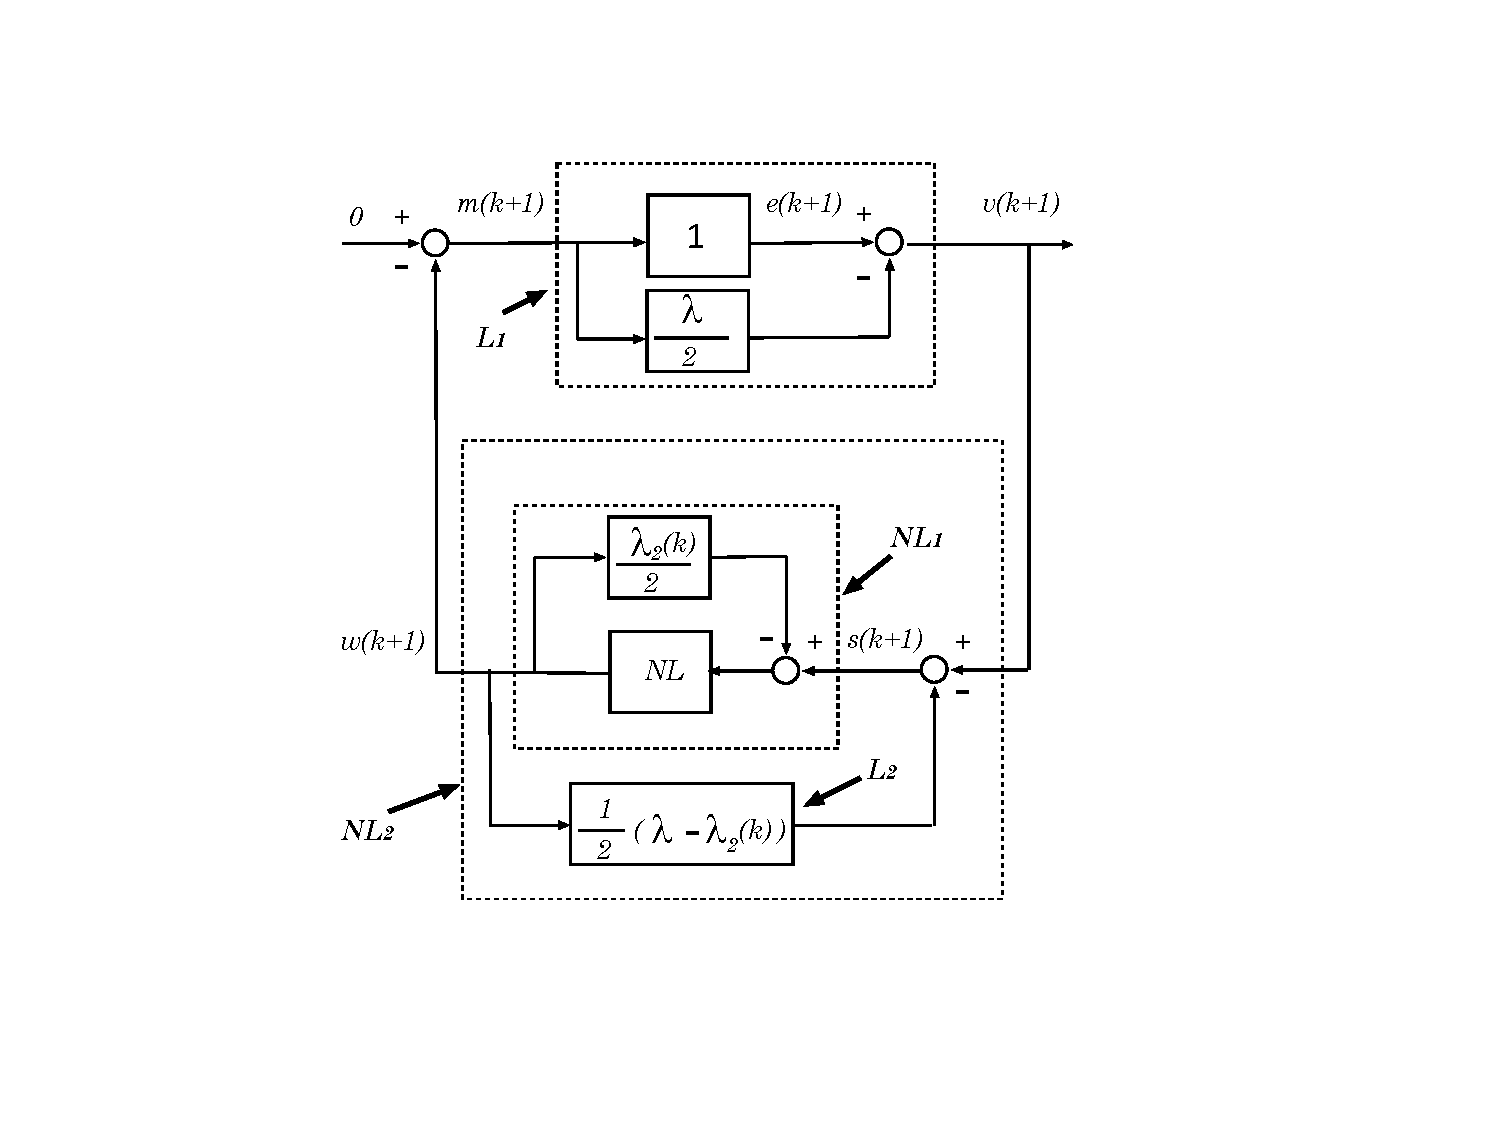
\includegraphics[width=\columnwidth]{figs_hyperstability}\\
        \end{figure}
    \end{columns}
\end{frame}

\begin{frame}
    \frametitle{Stability theorem proof, part 2}

    Because $\lambda - \lambda_2(j-1) \geq 0, \ j = -1,0,1,\ldots$, we have
    \begin{align*}
        -\bar{\gamma}^2 & \leq -\sum_{j=0}^k w(j) \Big[ s(j) + \frac{1}{2}(\lambda - \lambda_2(j-1)) w(j) \Big] \\
        & \leq -\sum_{j=0}^k w(j) s(j) \\
    \end{align*}
    \pause
    which implies that
    \begin{align*}
        \sum_{j=0}^k w(j) s(j) \leq \bar{\gamma}^2
    \end{align*}
\end{frame}

\begin{frame}
    \frametitle{Stability theorem proof, part 2}

    From part 1 of the stability theorem proof,
    \begin{align*}
        2 w(k) s(k) & = \tilde{\theta}_c^T(k) F^{-1}(k) \tilde{\theta}_c(k)
            - \lambda_1(k) \tilde{\theta}_c^T(k-1) F^{-1}(k-1) \tilde{\theta}_c(k-1) \\
        & \quad + \lambda_1(k) \Delta\theta_c^T(k) F^{-1}(k-1) \Delta\theta_c(k)
    \end{align*}
    \pause

    Since $0 < \underline{\lambda}_1 \leq \lambda_1(k) \leq 1$ and $F(k-1) \succ 0$, this implies that
    \begin{align*}
         2 w(k) s(k) & \geq \left[ \tilde{\theta}_c^T(k) F^{-1}(k) \tilde{\theta}_c(k)
            - \tilde{\theta}_c^T(k-1) F^{-1}(k-1) \tilde{\theta}_c(k-1) \right] \\
         & \quad + \underline{\lambda}_1 \Delta\theta_c^T(k) F^{-1}(k-1) \Delta\theta_c(k)
    \end{align*}
        
\end{frame}

\begin{frame}
    \frametitle{Stability theorem proof, part 2}    
    
    \begin{align*}
         2 w(k) s(k) & \geq \left[ \tilde{\theta}_c^T(k) F^{-1}(k) \tilde{\theta}_c(k)
            - \tilde{\theta}_c^T(k-1) F^{-1}(k-1) \tilde{\theta}_c(k-1) \right] \\
         & \quad + \underline{\lambda}_1 \Delta\theta_c^T(k) F^{-1}(k-1) \Delta\theta_c(k)
    \end{align*}
    \hrule{\hfill}
    
    which implies that
    \begin{align*}
        2 \bar{\gamma}^2 & \geq 2 \sum_{j=0}^k w(j) s(j) \\
        & \geq \sum_{j=0}^k \left[ \tilde{\theta}_c^T(j) F^{-1}(j) \tilde{\theta}_c(j)
            - \tilde{\theta}_c^T(j-1) F^{-1}(j-1) \tilde{\theta}_c(j-1) \right] \\
        & \quad + \sum_{j=0}^k \underline{\lambda}_1 \Delta \theta_c^T(j) F^{-1}(j-1) \Delta \theta_c(j)
    \end{align*}
\end{frame}

\begin{frame}
    \frametitle{Stability theorem proof, part 2}

    \vspace*{-\baselineskip}
    \begin{align*}
        2 \bar{\gamma}^2 & \geq \sum_{j=0}^k \left[ \tilde{\theta}_c^T(j) F^{-1}(j) \tilde{\theta}_c(j)
            - \tilde{\theta}_c^T(j-1) F^{-1}(j-1) \tilde{\theta}_c(j-1) \right] \\
        & \quad + \sum_{j=0}^k \underline{\lambda}_1 \Delta \theta_c^T(j) F^{-1}(j-1) \Delta \theta_c(j)
    \end{align*}
    \hrule{\hfill}
    
    \vspace*{-\baselineskip}
    \begin{align*}
        2 \bar{\gamma}^2 & = \tilde{\theta}_c^T(k) F^{-1}(k) \tilde{\theta}_c(k)
            - \tilde{\theta}_c^T(-1) F^{-1}(-1) \tilde{\theta}_c(-1) \\
        & \quad + \underline{\lambda}_1 \sum_{j=0}^k \Delta \theta_c^T(j) F^{-1}(j-1) \Delta \theta_c(j) \\
        & \geq - \tilde{\theta}_c^T(-1) F^{-1}(-1) \tilde{\theta}_c(-1)
            + \underline{\lambda}_1 \sum_{j=0}^k \Delta \theta_c^T(j) F^{-1}(j-1) \Delta \theta_c(j)
    \end{align*}
\end{frame}

\begin{frame}
    \frametitle{Stability theorem proof, part 2}

    Thus, we know that
    \begin{align*}
        \sum_{j=0}^k \Delta \theta_c^T(j) F^{-1}(j-1) \Delta \theta_c(j) \leq
            \frac{1}{ \underline{\lambda}_1 } 
            \left[ 2 \bar{\gamma}^2 + \tilde{\theta}_c^T(-1) F^{-1}(-1) \tilde{\theta}_c(-1) \right]
    \end{align*}
    \pause
    Since $F^{-1}(k) \succ 0 \ \forall k$, this implies that
    \begin{align*}
        \lim_{k \rightarrow \infty} \Delta \theta_c^T(k) F^{-1}(k-1) \Delta \theta_c(k) = 0
    \end{align*}
    \pause

    Since $\displaystyle \lambda_{min} (F^{-1}(k-1)) = \frac{1}{ \lambda_{max} (F(k-1)) } \geq \frac{1}{K_{max}} > 0$, this implies that
    \alignbox{
        \lim_{k \rightarrow \infty} \| \Delta \theta_c(k) \| = 0
    }
\end{frame}

\begin{frame}
    \frametitle{Stability theorem proof, part 2}

    Substituting the parameter update equation
    \begin{align*}
        \Delta \theta_c(k) = F(k-1) \phi(k-\drm) e(k)
    \end{align*}
    into
    \begin{align*}
        \lim_{k \rightarrow \infty} \Delta \theta_c^T(k) F^{-1}(k-1) \Delta \theta_c(k) = 0
    \end{align*}
    we obtain
    \begin{align*}
        \lim_{k \rightarrow \infty} \phi^T(k-\drm) F(k-1) \phi(k-\drm) e^2(k) = 0
    \end{align*}
    \pause
    Adding the equation $\displaystyle \lim_{k\rightarrow \infty} \lambda_1(k-1) e^2(k) = 0$ to this equation yields
    \begin{align*}
        \lim_{k \rightarrow \infty} [\lambda_1(k-1) + \phi^T(k-\drm) F(k-1) \phi(k-\drm)] e^2(k) = 0
    \end{align*}

\end{frame}

\begin{frame}
    \frametitle{Stability theorem proof, part 2}

    We know that
    \begin{align*}
        \lim_{k \rightarrow \infty} [\lambda_1(k-1) + \phi^T(k-\drm) F(k-1) \phi(k-\drm)] e^2(k) = 0
    \end{align*}

    $ \ $

    Since $\displaystyle e(k) = \frac{ \lambda_1(k-1) e^o(k) }{ \lambda_1(k-1) + \phi^T(k-\drm) F(k-1) \phi(k-\drm) } $, we have

    $ \ $

    \alignbox{
        \lim_{k \rightarrow \infty} \frac{ [\lambda_1(k-1) e^o(k)]^2 }
            { \lambda_1(k-1) + \phi^T(k-\drm) F(k-1) \phi(k-\drm) } = 0
    }

\end{frame}

\begin{frame}
    \frametitle{Stability theorem proof, part 2}

    Recall that $\eta_d(k) = r(k-\drm)$ and the control is given by
    \begin{align*}
        \hat{R}(q^{-1},k) u(k) = r(k) - \hat{S}(q^{-1},k) y(k)
    \end{align*}
    \pause
    We therefore see that
    \begin{align*}
        \eta_d(k+\drm) & = r(k) = \hat{R}(q^{-1},k) u(k) + \hat{S}(q^{-1},k) y(k) \\
        & = \phi^T(k) \hat{\theta}_c(k)
    \end{align*}
    \pause
    which allows us to say that
    \begin{align*}
        \epsilon(k) & = \eta(k) - \eta_d(k) = \phi^T(k-\drm) \tilde{\theta}_c(k-\drm) \\
        & = {\color{red} \phi^T(k-\drm) \tilde{\theta}_c(k-1) } + \phi^T(k-\drm) \Big[ \tilde{\theta}_c(k-\drm)
            - \tilde{\theta}_c(k-1) \Big] \\
        & = {\color{red} e^o(k)} + \phi^T(k-\drm) \Big[ \tilde{\theta}_c(k-\drm)
            - \tilde{\theta}_c(k-1) \Big]
    \end{align*}

\end{frame}

\begin{frame}
    \frametitle{Stability theorem proof, part 2}

    For convenience, define

    \begin{align*}
        \zeta(k) = \frac{\lambda_1(k-1) + \phi^T(k-\drm) F(k-1) \phi(k-\drm)}{\lambda_1^2(k-1)}
    \end{align*}
    In this notation, we know that $\displaystyle \lim_{k\rightarrow \infty} \frac{ [e^o(k)]^2 }{ \zeta(k) } = 0$
    \pause
    
    $\,$

    Since $0 < \lambda_1(k) \leq 1$ and $0 < K_{min} \leq \lambda_{min} (F(k)) \ \forall k$, we have
    \begin{gather*}
        \zeta(k) > \phi^T(k-\drm) F(k-1) \phi(k-\drm)
            \geq K_{min} \| \phi(k-\drm) \|^2 \geq 0
    \end{gather*}
    \paused
    
    \begin{gather*}
        \Rightarrow \frac{ \| \phi(k-\drm) \|^2 }{\zeta(k)} < \frac{1}{K_{min}}
    \end{gather*}

\end{frame}

\begin{frame}
    \frametitle{Stability theorem proof, part 2}

    By the Cauchy-Schwarz inequality,
    \begin{align*}
        & \left| \frac{ \phi^T(k-\drm) \Big[ \tilde{\theta}_c(k-\drm) - \tilde{\theta}_c(k-1) \Big] }
            { \sqrt{\zeta(k)} } \right| \\
        & \hspace{2.5cm} \leq \frac{ \| \phi(k-\drm) \| }{ \sqrt{\zeta(k)} } \|
            \tilde{\theta}_c(k-\drm) - \tilde{\theta}_c(k-1) \| \\
        & \hspace{2.5cm} \leq \frac{1}{ \sqrt{K_{min}} }
            \| \tilde{\theta}_c(k-\drm) - \tilde{\theta}_c(k-1) \|
    \end{align*}
    \pause
    
    The right-hand side of this inequality converges to zero because $\| \tilde{\theta}_c(k-\drm) - \tilde{\theta}_c(k-1) \|$ converges to zero.
    \pause
    
    Therefore
    \begin{align*}
        \lim_{k\rightarrow \infty} \frac{ \phi^T(k-\drm) \Big[ \tilde{\theta}_c(k-\drm) - \tilde{\theta}_c(k-1) \Big] }
            { \sqrt{\zeta(k)} } = 0
    \end{align*}

\end{frame}

\begin{frame}
    \frametitle{Stability theorem proof, part 2}

    Since $\epsilon(k) =  e^o(k) + \phi^T(k-\drm) \Big[ \tilde{\theta}_c(k-\drm) - \tilde{\theta}_c(k-1) \Big]$, we have
    \begin{align*}
        \lim_{k \rightarrow \infty} \frac{ \epsilon(k) }{ \sqrt{\zeta(k)} }
            & = \lim_{k \rightarrow \infty} \frac{ e^o(k) }{ \sqrt{\zeta(k)} } \\
        & \quad + \lim_{k \rightarrow \infty} \frac{ \phi^T(k-\drm) \Big[ \tilde{\theta}_c(k-\drm)
            - \tilde{\theta}_c(k-1) \Big] }{ \sqrt{\zeta(k)} } \\
        & = 0 + 0
    \end{align*}
    \pause

    Therefore
    \alignbox{
        \lim_{k \rightarrow \infty} \frac{ [\lambda_1(k-1) \epsilon(k)]^2 }
            { \lambda_1(k-1) + \phi^T(k-\drm) F(k-1) \phi(k-\drm) } = 0
    }

\end{frame}




\subsection{Part 3}
\begin{frame}
    \frametitle{Outline}
    \tableofcontents[currentsection]
\end{frame}

\begin{frame}
    \frametitle{Stability theorem proof, part 3}

    We want to prove that there exist $C_1 \geq 0, \ C_2 \geq 0$ such that
    \begin{align*}
        \| \phi(k-\drm) \| \leq C_1 + C_2 \max_{j \in \{0,\ldots,k\}} |\epsilon(j)|
    \end{align*}
    \paused
    
    We have the relationships
    \begin{align*}
        y(k) & = \frac{ q^{-\drm} B(q^{-1}) }{ A(q^{-1}) } u(k) = \frac{ B(q^{-1}) }{ A(q^{-1}) } u(k-\drm) \\
        \eta(k) & = A_c^{'}(q^{-1}) y(k) \\
        \epsilon(k) & = \eta(k) - \eta_d(k)
    \end{align*}
    which define $\epsilon(k)$ from $u(k)$ and $\eta_d(k)$.
    \pause
    
    We now invert these relationships, i.e.\ we reconstruct $u(k)$ from $\epsilon(k)$ and $\eta_d(k)$
\end{frame}

\begin{frame}
    \frametitle{Stability theorem proof, part 3}
        
    The inverted relationships are
    \begin{align*}
        u(k-\drm) & = \frac{ A(q^{-1}) }{ B(q^{-1}) } y(k) \\
        y(k) & = \frac{1}{ A_c^{'}(q^{-1}) } \eta(k) \\
        \eta(k) & = \epsilon(k) + \eta_d(k)
    \end{align*}
    \paused

    These relationships are shown in the block diagram
    \begin{figure}
        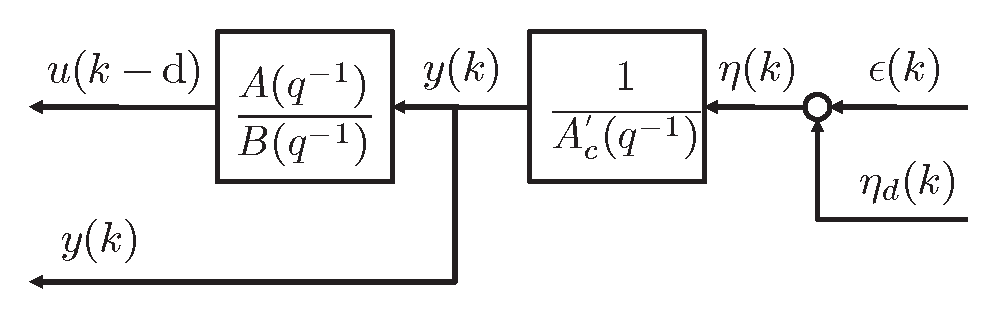
\includegraphics[width=8cm]{figs_bounded}\\
    \end{figure}
    
\end{frame}

\begin{frame}
    \frametitle{Stability theorem proof, part 3}

    \begin{figure}
        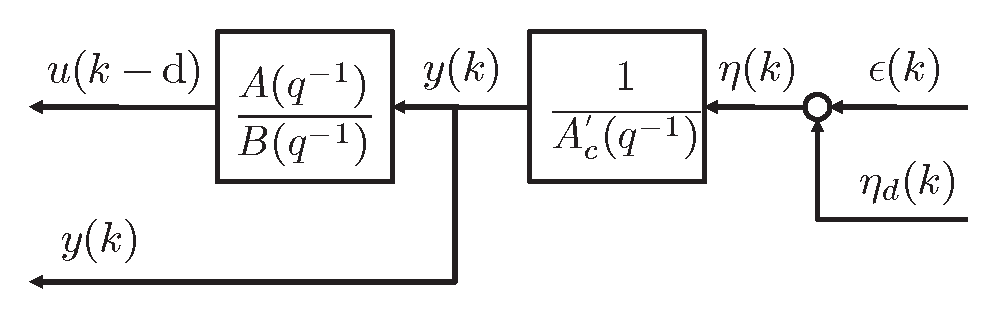
\includegraphics[width=8cm]{figs_bounded}\\
    \end{figure}
    \hrule{\hfill}
    
    Since $A_c^{'}(q^{-1})$ and $B(q^{-1})$ are anti-Schur, both blocks in the block diagram are causal and BIBO
    \pause
    
    Therefore, we can choose nonnegative $\bar{C}_{1u}$, $C_{2u}$, $\bar{C}_{1y}$, and $C_{2y}$ such that
    \begin{align*}
        |u(k-\drm)| & \leq \bar{C}_{1u} + C_{2u} \max_{j \leq k} |\eta(j)| \\
        |y(k)| & \leq \bar{C}_{1y} + C_{2y} \max_{j \leq k} |\eta(j)|
    \end{align*}

\end{frame}

\begin{frame}
    \frametitle{Stability theorem proof, part 3}

    \begin{align*}
        |u(k-\drm)| & \leq \bar{C}_{1u} + C_{2u} \max_{j \leq k} |\eta(j)| \\
        |y(k)| & \leq \bar{C}_{1y} + C_{2y} \max_{j \leq k} |\eta(j)|
    \end{align*}
    \hrule{\hfill}
    
    Assuming that $|\eta_d(k)| \leq \bar{\eta}_d$, the triangle inequality tells us that 
    \begin{align*}
        |\eta(j)| \leq |\eta_d(k)| + |\epsilon(k)| \leq \bar{\eta}_d + |\epsilon(k)|
    \end{align*}
    \paused
    
    Defining $C_{1u} = \bar{C}_{1u} + C_{2u} \bar{\eta}_d$ and $C_{1y} = \bar{C}_{1y} + C_{2y} \bar{\eta}_d$ we have
    \begin{align*}
        |u(k-\drm)| & \leq C_{1u} + C_{2u} \max_{j \leq k} |\epsilon(j)| \\
        |y(k)| & \leq C_{1y} + C_{2y} \max_{j \leq k} |\epsilon(j)|
    \end{align*}

\end{frame}

\begin{frame}
    \frametitle{Stability theorem proof, part 3}

    \begin{align*}
        |u(k-\drm)| & \leq C_{1u} + C_{2u} \max_{j \leq k} |\epsilon(j)| \\
        |y(k)| & \leq C_{1y} + C_{2y} \max_{j \leq k} |\epsilon(j)|
    \end{align*}
    \hrule{\hfill}
    
    Since $\displaystyle \max_{j \leq k-\ell} |\epsilon(j)| \leq \max_{j \leq k} |\epsilon(j)|$ for $\ell \geq 0$, we have
    \begin{align*}
        |u(k-\drm-\ell)| & \leq C_{1u} + C_{2u} \max_{j \leq k} |\epsilon(j)| \\
        |y(k-\drm-\ell)| & \leq C_{1y} + C_{2y} \max_{j \leq k} |\epsilon(j)|
    \end{align*}
    for all $\ell \geq 0$

\end{frame}

\begin{frame}
    \frametitle{Stability theorem proof, part 3}

    \vspace*{-\baselineskip}
    \begin{align*}
        |u(k-\drm-\ell)| & \leq C_{1u} + C_{2u} \max_{j \leq k} |\epsilon(j)| \\
        |y(k-\drm-\ell)| & \leq C_{1y} + C_{2y} \max_{j \leq k} |\epsilon(j)|
    \end{align*}
    \hrule{\hfill}

    Using the triangle inequality, we have
    \begin{align*}
        & \| \phi(k-\drm) \| \leq \sum_{j=0}^{n_s} \left| y(k-\drm-j) \right|
            + \sum_{i=0}^{n_r} \left| u(k-\drm-i) \right| \\
        & \hspace{.5cm} \begin{aligned}
        & \leq \sum_{j=0}^{n_s} \left( C_{1y} + C_{2y} \max_{\ell \leq k} |\epsilon(\ell)| \right)
            + \sum_{i=0}^{n_r} \left( C_{1u} + C_{2u} \max_{\ell \leq k} |\epsilon(\ell)| \right)% \\
%        & \leq \left[ (n_s+1) C_{1y} + (n_r+1) C_{1u} \right] \\
%        & \quad + \left[ (n_s+1) C_{2y} + (n_r+1) C_{2u} \right] \max_{j \leq k} |\epsilon(j)|
        \end{aligned}
    \end{align*}
    \paused
    
    Therefore
    \alignbox{
        \| \phi(k-\drm) \| & \leq \left[ (n_s+1) C_{1y} + (n_r+1) C_{1u} \right] \\
        & \quad + \left[ (n_s+1) C_{2y} + (n_r+1) C_{2u} \right] \max_{j \leq k} |\epsilon(j)|
    }

\end{frame}





\subsection{Part 4}
\begin{frame}
    \frametitle{Outline}
    \tableofcontents[currentsection]
\end{frame}

\begin{frame}
    \frametitle{Stability theorem proof, part 4}

    We want to prove Goodwin's technical lemma, which states that $\| \phi(k) \|$ remains bounded and
    \begin{align*}
        \lim_{k \rightarrow \infty} \epsilon(k) = 0
    \end{align*}
    \pause

    This proof will be done in three steps:
    \begin{enumerate}
        \item
        Show that $\epsilon(k)$ remains bounded
        
        \item
        Show that $\| \phi(k) \|$ remains bounded
        
        \item
        Show that $\epsilon(k) \longrightarrow 0$
    \end{enumerate}
\end{frame}

\begin{frame}
    \frametitle{Stability theorem proof, part 4, step 1 ($\epsilon(k)$ bounded)}    

    Recall from part 2 that
    \begin{align*}
        \lim_{k \rightarrow \infty} \frac{ [\lambda_1(k-1) \epsilon(k)]^2 }
            { \lambda_1(k-1) + \phi^T(k-\drm) F(k-1) \phi(k-\drm) } = 0
    \end{align*}
    \pause
    
    Since $0 < \underline{\lambda}_1 \leq \lambda_1(k) \leq 1$ \\
    and $0 < \lambda_{min}(F(k-1)) \leq \lambda_{max}(F(k-1)) \leq K_{max}$ \\
    we have
    \begin{multline*}
        \left| \frac{ [\lambda_1(k-1) \epsilon(k)]^2 }
            { \lambda_1(k-1) + \phi^T(k-\drm) F(k-1) \phi(k-\drm) } \right| \\
        \geq \frac{ \underline{\lambda}_1^2 \epsilon^2(k) }{ 1 + K_{max} \| \phi(k-\drm) \|^2 } > 0
    \end{multline*}
    
\end{frame}

\begin{frame}
    \frametitle{Stability theorem proof, part 4, step 1 ($\epsilon(k)$ bounded)}
    
    \begin{multline*}
        \left| \frac{ [\lambda_1(k-1) \epsilon(k)]^2 }
            { \lambda_1(k-1) + \phi^T(k-\drm) F(k-1) \phi(k-\drm) } \right| \\
        \geq \frac{ \underline{\lambda}_1^2 \epsilon^2(k) }{ 1 + K_{max} \| \phi(k-\drm) \|^2 } > 0
    \end{multline*}
    \hrule{\hfill}

    For convenience, we define $\displaystyle \overline{\epsilon}(k) \ \max_{j\leq k} |\epsilon(j)|$
    \pause
    
    $\, $
    
    From part 3, we have that $\| \phi(k-\drm) \|^2 \leq [C_1 + C_2 \overline{\epsilon}(k)]^2$, which implies that
    \begin{multline*}
        \left| \frac{ [\lambda_1(k-1) \epsilon(k)]^2 }
            { \lambda_1(k-1) + \phi^T(k-\drm) F(k-1) \phi(k-\drm) } \right| \\
        \geq \frac{ \underline{\lambda}_1^2 \epsilon^2(k) }{ 1 + K_{max} [C_1 + C_2 \overline{\epsilon}(k)]^2 } > 0
    \end{multline*}    

    
\end{frame} 

\begin{frame}
    \frametitle{Stability theorem proof, part 4, step 1 ($\epsilon(k)$ bounded)}

    \begin{multline*}
        \left| \frac{ [\lambda_1(k-1) \epsilon(k)]^2 }
            { \lambda_1(k-1) + \phi^T(k-\drm) F(k-1) \phi(k-\drm) } \right| \\
        \geq \frac{ \underline{\lambda}_1^2 \epsilon^2(k) }{ 1 + K_{max} [C_1 + C_2 \overline{\epsilon}(k)]^2 } > 0
    \end{multline*}
    \hrule{\hfill}
        
    Since 
    \begin{align*}
        \lim_{k \rightarrow \infty} \frac{ [\lambda_1(k-1) \epsilon(k)]^2 }
            { \lambda_1(k-1) + \phi^T(k-\drm) F(k-1) \phi(k-\drm) } = 0
    \end{align*}
    we have
    \begin{align*}
        \lim_{k \rightarrow \infty} \frac{ \underline{\lambda}_1^2 \epsilon^2(k) }
            { 1 + K_{max} [C_1 + C_2 \overline{\epsilon}(k)]^2 } = 0
    \end{align*}

\end{frame} 

\begin{frame}
    \frametitle{Stability theorem proof, part 4, step 1 ($\epsilon(k)$ bounded)}

    \begin{align*}
        \lim_{k \rightarrow \infty} \frac{ \underline{\lambda}_1^2 \epsilon^2(k) }
            { 1 + K_{max} [C_1 + C_2 \overline{\epsilon}(k)]^2 } = 0
    \end{align*}
    \hrule{\hfill}

    Whenever $\displaystyle |\epsilon(k)| = \overline{\epsilon}(k) \geq 1$, we have
    \begin{align*}
        0 & < \frac{ 1 + K_{max} [C_1 + C_2 \overline{\epsilon}(k)]^2 }{ \underline{\lambda}_1^2 \overline{\epsilon}^2(k) } \\
        & = \frac{ 1 + K_{max} C_1^2 }{ \underline{\lambda}_1^2 \overline{\epsilon}^2(k) }
            + \frac{ 2 K_{max} C_1 C_2 }{ \underline{\lambda}_1^2 \overline{\epsilon}(k) } 
            + \frac{ K_{max} C_2^2 }{ \underline{\lambda}_1^2 } \\
        & \leq \frac{1}{\underline{\lambda}_1^2 } [1 + K_{max} C_1^2 + 2 K_{max} C_1 C_2 + K_{max} C_2^2]
    \end{align*}
    \paused
    
    This implies that whenever $\displaystyle |\epsilon(k)| = \overline{\epsilon}(k) \geq 1$, we have
    \begin{align*}
        \frac{ \underline{\lambda}_1^2 \epsilon^2(k) }{ 1 + K_{max} [C_1 + C_2 \overline{\epsilon}(k)]^2 } 
            \geq \frac{ \underline{\lambda}_1^2 }{ 1 + K_{max} [C_1 + C_2]^2 } > 0
    \end{align*}

\end{frame} 

\begin{frame}
    \frametitle{Stability theorem proof, part 4, step 1 ($\epsilon(k)$ bounded)}

    Whenever $\displaystyle |\epsilon(k)| = \overline{\epsilon}(k) \geq 1$, we have
    \begin{align*}
        \frac{ \underline{\lambda}_1^2 \epsilon^2(k) }{ 1 + K_{max} [C_1 + C_2 \overline{\epsilon}(k)]^2 }
            \geq \frac{ \underline{\lambda}_1^2 }{ 1 + K_{max} [C_1 + C_2]^2 } > 0
    \end{align*}
    \hrule{\hfill}
    
    Since
    \begin{align*}
        \lim_{k \rightarrow \infty} \frac{ \underline{\lambda}_1^2 \epsilon^2(k) }
            { 1 + K_{max} [C_1 + C_2 \overline{\epsilon}(k)]^2 } = 0
    \end{align*}
    there can only be a finite number of values of $k$ such that $\displaystyle |\epsilon(k)| = \overline{\epsilon}(k) = \max_{j\leq k} |\epsilon(j)| \geq 1$.
    \pause
    
    $\,$
    
    Therefore, 
    \alignbox{
        \epsilon(k) \textrm{ remains bounded}
    }
    
\end{frame}

\begin{frame}
    \frametitle{Stability theorem proof, part 4, step 2 ($\phi(k)$ bounded)}

    Recall from part 3 that
    \begin{align*}
        \| \phi(k-\drm) \| & \leq C_1 + C_2 \max_{j \leq k} |\epsilon(j)|
    \end{align*}
    \pause
    
    Since $\epsilon(k)$ remains bounded, we immediately see that
    \alignbox{
        \phi(k) \textrm{ remains bounded}
    }

\end{frame}

\begin{frame}
    \frametitle{Stability theorem proof, part 4, step 3 ($\epsilon(k) \longrightarrow 0$)}

    Recall from part 2 that
    \begin{align*}
        \lim_{k \rightarrow \infty} \frac{ \epsilon^2(k) }{ \zeta(k) } = 0
    \end{align*}
    where
    \begin{align*}
        \zeta(k) = \frac{\lambda_1(k-1) + \phi^T(k-\drm) F(k-1) \phi(k-\drm)}{\lambda_1^2(k-1)}
    \end{align*}
    \pause
    
    Therefore, if we can show that $\zeta(k)$ remains bounded, it must be true that $\epsilon(k) \longrightarrow 0$

\end{frame}

\begin{frame}
    \frametitle{Stability theorem proof, part 4, step 3 ($\epsilon(k) \longrightarrow 0$)}

    Since $0 < \underline{\lambda}_1 \leq \lambda_1(k) \leq 1$ \\
    and $0 < \lambda_{min}(F(k-1)) \leq \lambda_{max}(F(k-1)) \leq K_{max}$ \\
    we have
    \begin{align*}
        |\zeta(k)| & = \left| \frac{\lambda_1(k-1) + \phi^T(k-\drm) F(k-1) \phi(k-\drm)}{\lambda_1^2(k-1)} \right| \\
        & \leq \frac{ 1 + K_{max} \| \phi(k-\drm) \|^2 }{ \underline{\lambda}_1^2 }
    \end{align*}
    \pause
    
    Since the right-hand side is bounded, we see that $\zeta(k)$ remains bounded.
    \pause
    
    Therefore
    \alignbox{
        \lim_{k \rightarrow \infty} \epsilon(k) = 0
    }

\end{frame}





\subsection{Part 5}
\begin{frame}
    \frametitle{Outline}
    \tableofcontents[currentsection]
\end{frame}


\begin{frame}
    \frametitle{Stability theorem proof, part 5}

    Recall from part 2 that
    \begin{align*}
        \lim_{k \rightarrow \infty} \frac{ [e^o(k)]^2 }{ \zeta(k) } = 0
    \end{align*}
    where
    \begin{align*}
        \zeta(k) = \frac{\lambda_1(k-1) + \phi^T(k-\drm) F(k-1) \phi(k-\drm)}{\lambda_1^2(k-1)}
    \end{align*}
    \pause
    
    We have already shown that $\zeta(k)$ is bounded
    \pause
    
    Therefore
    \alignbox{
        \lim_{k \rightarrow \infty} e^o(k) = 0
    }

\end{frame}




\end{document} 
